\documentclass[border=3pt]{standalone}
% Preâmbulo compartilhado pelos diagramas TikZ da aula 13 (SLAM com EKF)
\usepackage[T1]{fontenc}
\usepackage[utf8]{inputenc}
\usepackage{lmodern}
\usepackage{amsmath}
\usepackage{xcolor}
\usepackage{tikz}
\usetikzlibrary{arrows.meta,angles,quotes,decorations.pathmorphing,decorations.pathreplacing,calc,
                positioning,shapes.geometric,shapes.misc,backgrounds,fit,
                math}

% Paleta (mesma dos SVGs originais)
\definecolor{dblue}{HTML}{2A5B8C}
\definecolor{dorange}{HTML}{B3541E}
\definecolor{dgreen}{HTML}{4A7C59}
\definecolor{dred}{HTML}{9C4B4B}
\definecolor{dcream}{HTML}{F4F1EA}
\definecolor{dshade}{HTML}{DDD7C9}

% Função gaussiana (não normalizada por padrão de escala visual)
\pgfmathdeclarefunction{gauss}{3}{%
  \pgfmathparse{1/(#3*sqrt(2*pi))*exp(-((#1-#2)^2)/(2*#3^2))}%
}

% Estilos comuns (prefixo d... para não colidir com chaves internas do pgf)
\tikzset{
  >={Stealth[length=2mm]},
  dguide/.style={gray!55, dashed, line width=0.4pt},
  daxis/.style={gray!60, line width=0.7pt, ->},
  dbody/.style={fill=black!3, draw=black!80, line width=1pt},
  dacc/.style={draw=dblue, line width=1pt},
  dlbl/.style={black!55, font=\small},
  dsub/.style={black!45, font=\footnotesize},
  dstate/.style={circle, draw=black!80, fill=dcream, line width=1pt,
                 minimum size=17mm, font=\large, inner sep=1pt},
  dobs/.style={circle, draw=black!80, fill=dshade, line width=1pt,
               minimum size=14mm, font=\large, inner sep=1pt},
  dbox/.style={rounded corners=2pt, draw=black!80, fill=dcream, line width=1pt,
               align=center, inner sep=6pt},
  dop/.style={circle, draw=black!80, fill=white, line width=1pt,
              minimum size=6mm, inner sep=0pt, font=\small},
  dtrans/.style={->, dblue, line width=1pt},
  dmeas/.style={->, dorange, line width=1pt},
  dcurve/.style={line width=1pt, dblue},
  dcurveb/.style={line width=1.4pt, dorange},
}

\begin{document}
\hyphenpenalty=10000 \exhyphenpenalty=10000 \tolerance=9999 \emergencystretch=3em
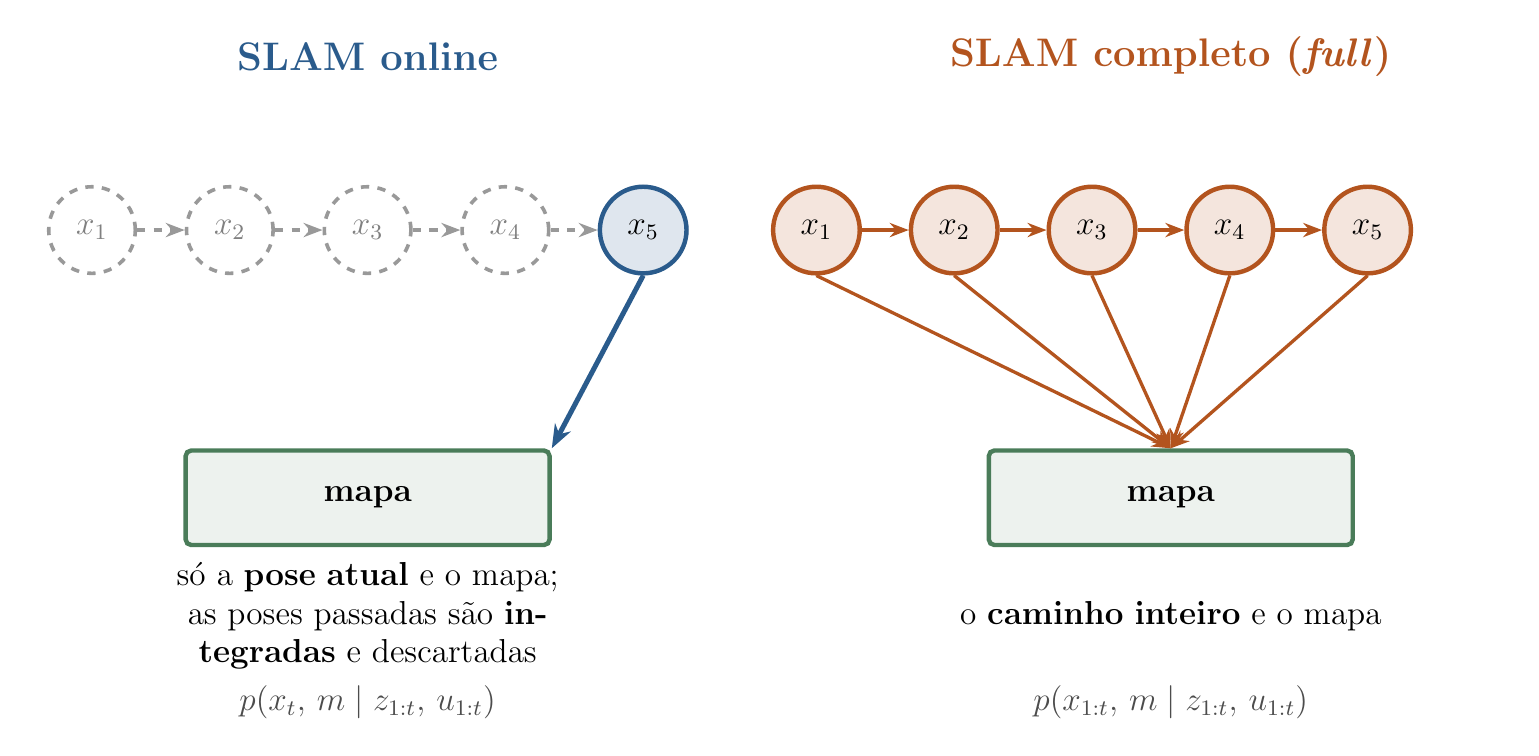
\begin{tikzpicture}[x=1cm,y=1cm]
\tikzset{p/.style={circle, draw=dblue, fill=dblue!15, line width=1.6pt, minimum size=1.1cm, font=\large},
        f/.style={circle, draw=black!40, dashed, fill=white, line width=1.3pt, minimum size=1.1cm, font=\large, text=black!50},
        mp/.style={dbox, draw=dgreen, fill=dgreen!10, line width=1.6pt, text width=4.2cm, minimum height=1.2cm, font=\large\bfseries}}
\node[font=\Large\bfseries, dblue] at (4.4,8.6) {SLAM online};
\node[font=\Large\bfseries, dorange] at (14.6,8.6) {SLAM completo (\emph{full})};
\foreach \i in {1,2,3,4,5} {
  \node[f] (a\i) at ({0.9+(\i-1)*1.75},6.4) {$x_\i$};
  \node[p, draw=dorange, fill=dorange!15] (b\i) at ({11.1+(\i-1)*1.75-1.0},6.4) {$x_\i$};
}
\node[p] (a5) at (7.9,6.4) {$x_5$};
\foreach \i/\j in {1/2,2/3,3/4,4/5} {
  \draw[black!40, dashed, line width=1.2pt, -{Stealth[length=2.4mm]}] (a\i) -- (a\j);
  \draw[dorange, line width=1.4pt, -{Stealth[length=2.4mm]}] (b\i) -- (b\j);
}
\node[mp] (ma) at (4.4,3.0) {mapa};
\node[mp] (mb) at (14.6,3.0) {mapa};
\draw[dblue, line width=1.8pt, -{Stealth[length=3mm]}] (a5.south) -- (ma.north east);
\foreach \i in {1,2,3,4,5} {\draw[dorange, line width=1.2pt, -{Stealth[length=2.4mm]}] (b\i.south) -- (mb.north);}
\node[font=\large, text width=8.4cm, align=center] at (4.4,1.5) {só a \textbf{pose atual} e o mapa;\\ as poses passadas são \textbf{integradas} e descartadas};
\node[font=\large, text width=8.4cm, align=center] at (14.6,1.5) {o \textbf{caminho inteiro} e o mapa};
\node[font=\large, black!70] at (4.4,0.4) {$p(x_t,\, m \mid z_{1:t},\, u_{1:t})$};
\node[font=\large, black!70] at (14.6,0.4) {$p(x_{1:t},\, m \mid z_{1:t},\, u_{1:t})$};
\end{tikzpicture}
\end{document}
